\documentclass{article}
\usepackage{graphicx}
\usepackage{array}
\usepackage{natbib}
\usepackage[margin=1in]{geometry}
\usepackage{amsmath}
\newcommand{\norm}[1]{\left\lVert#1\right\rVert}
%\usepackage{titlesec}
%\titleclass{\section}{top}
%\newcommand\sectionbreak{\clearpage}
\date{}
\makeatletter
\renewcommand\paragraph{\@startsection{paragraph}{4}{\z@}%
	{-2.5ex\@plus -1ex \@minus -.25ex}%
	{1.25ex \@plus .25ex}%
	{\normalfont\normalsize\bfseries}}
\makeatother
\setcounter{secnumdepth}{4}
\setcounter{tocdepth}{4}

\begin{document}
	\title{Methods for improving and characterizing gene families}
	\maketitle
	\tableofcontents
	\begin{abstract}
	Gene families are groups of genes that have evolved from single common ancestral gene present in the common ancestor of a given set of species. Studying evolution of genes in the families helps in inferring evolution of species and in detecting evolutionarily/funtionally equivalent regions between multiple different genomes. Current gene family clustering methods can produce non-optimal families that could be under-clustered (missing sequences) or over-clustered (containing sequences from more than one family). This project presents methods for analyzing gene families - for over- and under-clustering and by other characteristics, after they have been built using existing family building methods. The proposed methods include (1) a pair classification based approach for detecting and correcting under-clustered families; (2) tree-based methods that assess families based on expected phylogenetic toplogy; (3) domain composition methods that assess families based on domains detected in the sequences in a family; (4) species composition methods that assess families based on expected species in a family, relative to a model of gene duplications and speciations and (5) family sets comparison workflow for obtaining consensus families from multiple family sets built using different methods. Finally, the high-quality gene families from legume species, obtained using the proposed methods, are first divided into different groups based on their sizes and each group is characterized using Gene Ontology enrichment analysis.  
	\end{abstract}
	
	\section{Introduction}
		\subsection{Gene families}
		Gene families or orthologous groups - with respect to a given set of species - are clusters of genes that have originated from a single ancestral gene present in the common ancestor of the given set of species. Therefore, gene families contain genes that have diverged due to speciation or duplication after the divergence node of earliest diverging species. Accordingly, genes within the families are either orthologs or in-paralogs (duplication after the common ancestral node) \citep{fitch1970distinguishing,fitch2000homology, sonnhammer2002orthology}. Gene families are mainly used to infer orthology and paralogy among genes from the given set of species.
		
		Clustering genes into families helps in capturing evolutionary information from multiple species for studying the divergence or conservation of particular biological functions, with respect to given set of species. Gene families can also be used for identification of candidates drug/vaccine development in case of parasites like \textit{Plasmodium falciparum} which causes malaria in humans \citep{gardner2002genome,kissinger2002plasmodium,whetzel2005plasmodb}. Gene families have also been used for annotation of newly sequenced genomes and for anti-bacterial drug development by cross-referencing functional information from multiple species \citep{tatusov1997genomic,galperin1999searching,natale2000towards,natale2000using,forterre2002hot}
		
		\subsection{Improving and characterizing gene families}
		 Existing family building algorithms can be divided into 2 main categories, viz: alignment-based clustering approaches and tree based approaches. The clusters of Orthologous Groups (COG) database is one of the earliest widely-used collections of gene families \citep{tatusov2000cog,tatusov2001cog}. The orthologous groups in the COG database were identified based on reciprocal best hits from all-against-all BLAST searches using complete proteomes from five major lineages - Gram-negative bacteria, Gram-positive bacteria, Cyanbacteria, Archea, and Eukarya. The alignment-based clustering approaches either operate on individual pairs of species and then expand to multiple species - for example MultiParanoid (Inparanoid), OMA \citep{alexeyenko2006automatic,remm2001automatic,roth2008algorithm,altenhoff2010oma} - or attempt to infer families directly from multiple species with the common ancestor of given set of species as a reference;  OrthoMCL, OrthoFinder \citep{li2003orthomcl,emms2015orthofinder}. Tree-based methods compare the gene trees with the species trees using tree reconciliation methods for building gene families \citep{li2006treefam,van2007orthology,wapinski2007automatic,hubbard2006ensembl,dehal2006phylogenomic}.
		  
		 While many of the families produced by existing methods may be "correct", many non-optimal families could be produced due to under-clustering or over-clustering. Under-clustered families are those families that may have been fragmented by the clustering method (missing sequences). Over-clustered families are those families that may been produced due to merging of two or more closely related families. Also, a significant number of sequences can remain un-clustered and could be wrongly considered as singletons or orphan genes. 
		
		Therefore, it is important to analyze and assess the accuracy of families constructed using any method. Here, I propose a suite of methods and tools for improving under-clustered/over-clustered gene families, and for characterizing true and consistent families.
		
		\subsection{Gene families in legumes}
		The legume family (Fabaceae) consists of 750 genera and 19,500 species of flowering plants, making the third largest family of flowering plants \citep{lewis2005legumes}. The family is broadly divided into four major lineages viz. Papilionoideae, Mimosoideae-Cassiinae-Caesalpinieae (MCC), Detarieae and Cercideae, out of which the Papilionoideae is the largest. The Papilionoid sub-family includes species like \textit{Arachis hypogaea} (cultivated peanut), \textit{Cajanus cajan} (pigeonpea), \textit{Cicer arietinum} (chickpea), \textit{Glycine max} (soybean), \textit{Lotus japonicus} (Lotus), \textit{Lupinus angustifolius} (narrow-leafed lupin), \textit{Medicago truncatula} (barrel medic), \textit{Phaseolus vulgaris} (common bean), \textit{Trifolium pratense} (red clover), \textit{Vigna angularis} (adzuki bean), \textit{Vigna radiata} (mungbean) and \textit{Vigna unguiculata} (Cowpea).
		
		An ancient Whole Genome Duplication (WGD) has occurred in common ancestor of the Papilionoid sub-family around 55 Ma. \citep{blanc2004functional,schlueter2004mining,pfeil2005placing,cannon2006legume,bertioli2009analysis,cannon2014multiple}. In addition, the  lineages such as \textit{Glycine} and \textit{Lupin} have also undergone independent lineage specific WGDs \citep{cannon2014multiple,Kroc2014} 
		
		Approximately 17k-18k gene families were obtained using a Ks-based (synonymous substitutions per site) family building procedure from the Papilionoid species proteomes. Additionally, for comparison, a different set of 20k families was also obtained from Papilionoid species using the OthroFinder method \citep{emms2015orthofinder}.
		
		\subsection{Specific objectives}
			\begin{enumerate}
				\item Develop pair classification based methods for detecting and improving under-clustered gene families.
				
				\item Develop tree based, domain composition and species composition based methods for detecting  and improving over-clustered gene families.
				
				\item Develop a workflow for building consensus families from multiple family sets.
				
				\item Biological characterization of gene families for a set of species in the legume plant family.
			\end{enumerate}
		
		\pagebreak

	\section{Objective 1: Develop pair classification based methods for detecting under-clustered gene families} 
	This scoring method leverages the basic evolutionary property of gene families - all the sequences in the family must have diverged at/after the separation of earliest diverging species and none of the sequences outside the family have diverged in the family. Accordingly, for a given family, this method attempts to separate pairs from the family, from pairs where one sequence is in the family and other is outside the family. The separation statistics tell how well a given family of sequences can be circumscribed from closest non-family sequences.This can provide an indication of family completeness.
		\subsection{Methods}
			\subsubsection{Family searching and collecting closest non-family sequences}
			All the sequences from any given family are searched against the combined database of all proteomes from all the species under study (the sequence space). With each family sequence as query, all the hits that match the query better than the worst matching family hit (other than the query) are collected into a list. A combined list of hits, using each family sequence as a query, is obtained which is expected to contain both family and non-family sequences (Figure ~\ref{fig:collecting_non_fam_seqs}).
			
			The phmmer program from HMMER package \citep{eddy1992hmmer} is used for searching families against the sequence space database. The ranking of hits for finding the worst matching family hit is the same ranking given by the phmmer search results. 
			\begin{figure}
				\fbox{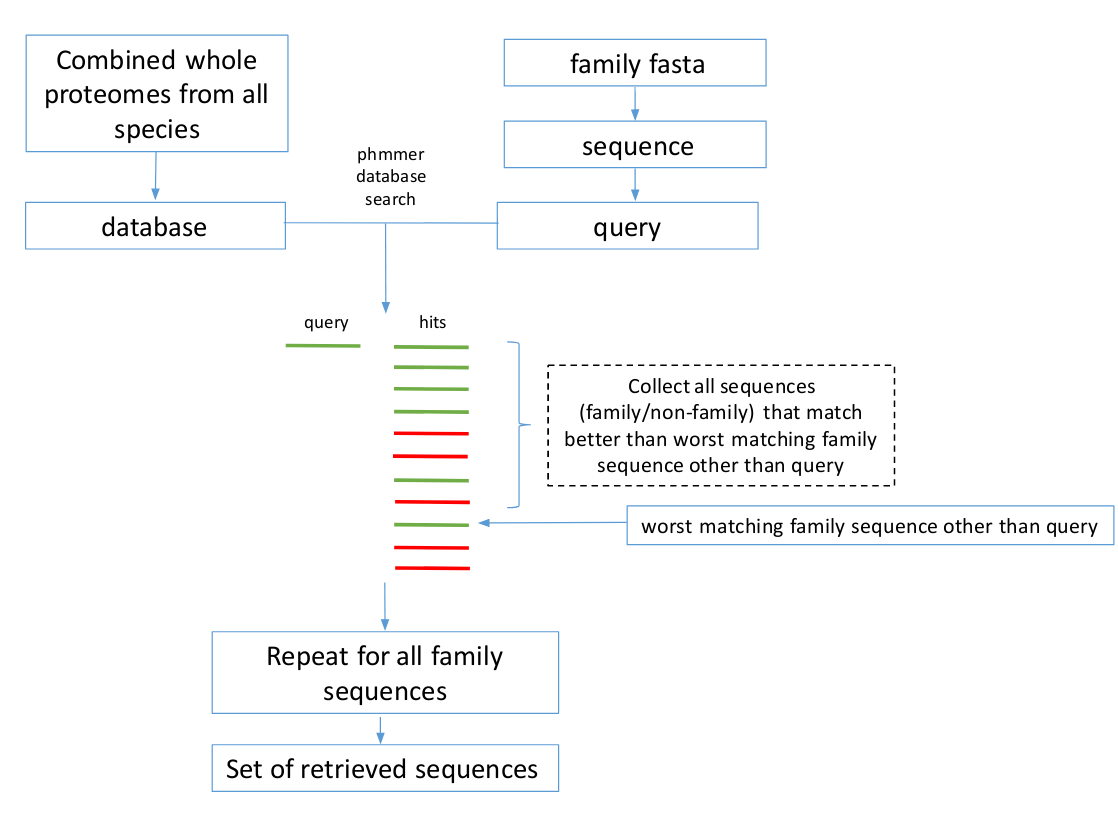
\includegraphics[width=\linewidth]{figures/collecting_non_fam_seqs.png}}
				\caption{Collecting closest non-family sequences}
				\label{fig:collecting_non_fam_seqs}
			\end{figure}
			
			\subsubsection{Forming family and non-family pairs}
			The combined list of family and non-family sequences obtained in the previous step is used to form family and non-family pairs (Figure ~\ref{fig:forming_pairs}). The family pairs are those that form exclusively between the original family members and the non-family pairs are those that form between the family and non-family members. The family pairs are labeled as positive pairs and the non-family pairs were labeled as the negative pairs.
			
			\begin{figure}
				\fbox{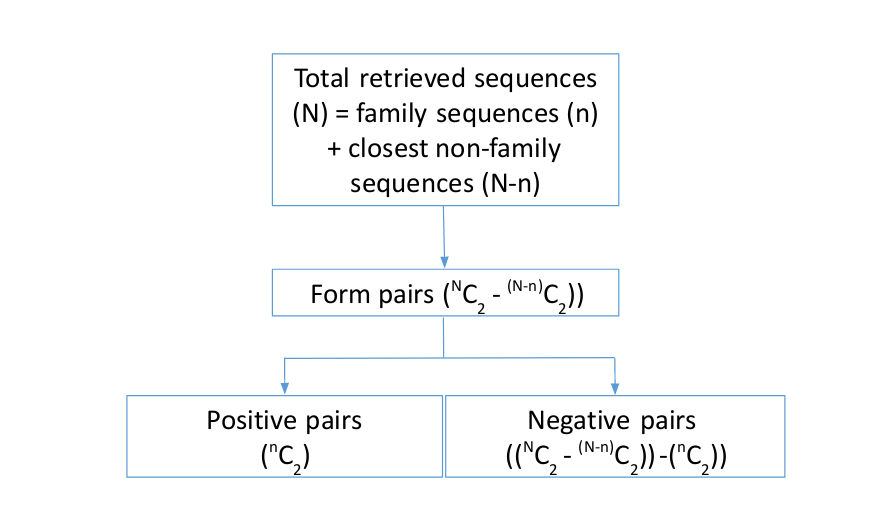
\includegraphics[width=\linewidth]{figures/forming_pairs.png}}
				\caption{Forming positive and negative pairs from family and non-family sequences}
				\label{fig:forming_pairs}
			\end{figure}
			
			\subsubsection{Model building and assessing classification performance}
			HMM based pair classification models are built to classify the family and non-family pairs, and 10 iterations of repeated test-train split strategy are used to assess the classification performance (Figure ~\ref{fig:train_classify1}). For each iteration, the set of family+non-family pairs are randomly split into training and test split. The pair classification model is trained on the training split and tested on the unseen test split. To train the HMM model on positive pairs in the training split, consensus sequences of the positive pairs are used. To test the model on pairs in the test split, individual sequences of the pairs are first aligned to the trained HMM model and alignment scores for both the sequences are obtained. The test pair is predicted as a positive pair if both the alignment scores are greater than or equal to a specified score cutoff.
			
			The Precision-Recall (PR) curve for the positive class is obtained using the combined predictions from all the 10 test-train split iterations. The test pair alignment scores from all the iterations are consolidated (Figure ~\ref{fig:train_classify2}) and used for calculating precision (TP/TP+FP), recall (TP/TP+FN) and F1-score (harmonic mean: 2*(precision*recall)/(precision+recall)) values for specified score cutoffs, where TP, FP and FN are the number True Positive, False Positive and False Negative pairs, respectively. Different precision and recall values are obtained for a range of score cutoffs starting from most stringent to least stringent. The precision values are plotted against the recall values to obtain the PR-curve \citep{davis2006relationship}. The area under the PR-curve (PR-AUC) is calculated using the trapezoidal rule. Other classification metrics such as the precision and recall values observed at the best F1-score and the score cutoff which gives the best F1-score are also reported. The lowest score observed for the positive class is also reported as the lowest score cutoff with respect to the given family. 
			
			An example of PR-curve plot for a hypothetical gene family is shown in Figure ~\ref{fig:test_PR-curve}. Each point on the curve corresponds to an alignment score cutoff with score cutoffs decreasing from left to right. The highest score cutoffs on the left produce classifications with highest precision (low FP) but lowest recall (high FN). Conversely, lowest score cutoffs on the right produce classifications with lowest precision but highest recall. An F1-score can be calculated for each point (precision, recall) on the curve as the harmonic mean of precision and the corresponding recall value. The point on the curve with the highest F1-score is the point where optimal values of precision and recall exist. This point represents the best classification performance for the family and the corresponding alignment score is the score cutoff that gives the best classification performance for the family.
			
			\begin{figure}
				\fbox{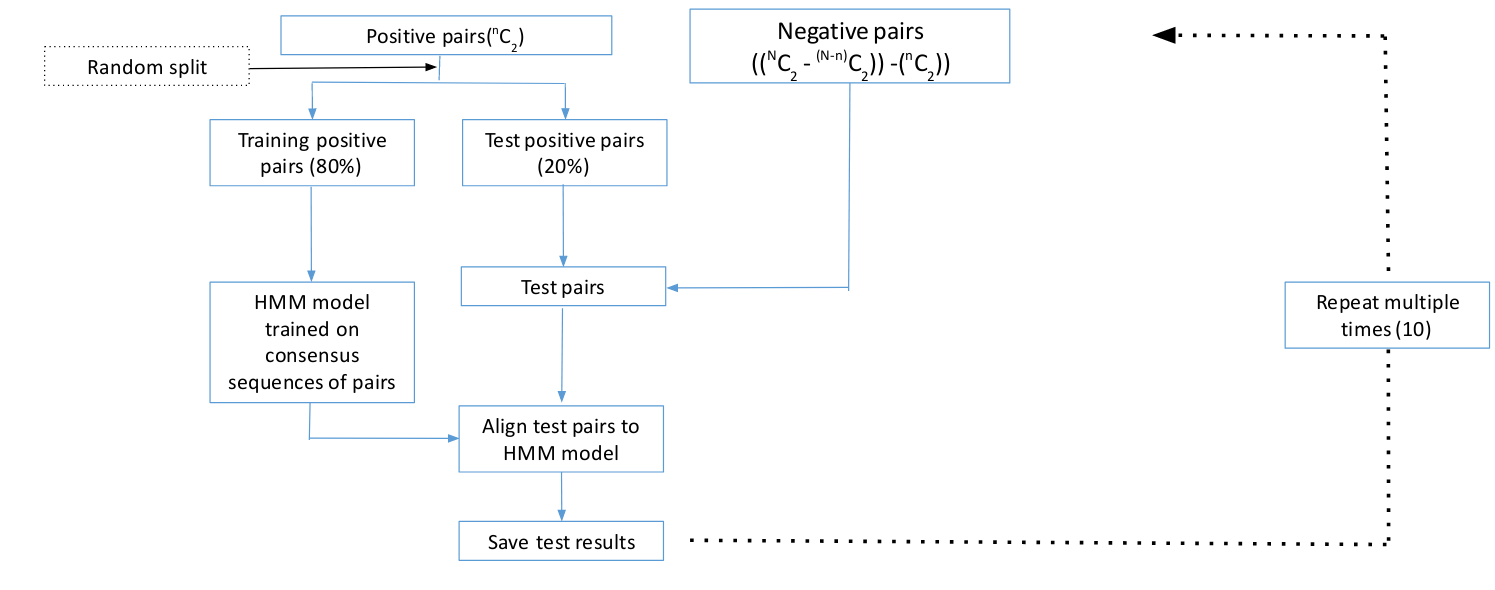
\includegraphics[width=\linewidth]{figures/train_classify1.png}}
				\caption{Training pair classification models for a family}
				\label{fig:train_classify1}
			\end{figure}
			
			\begin{figure}
				\fbox{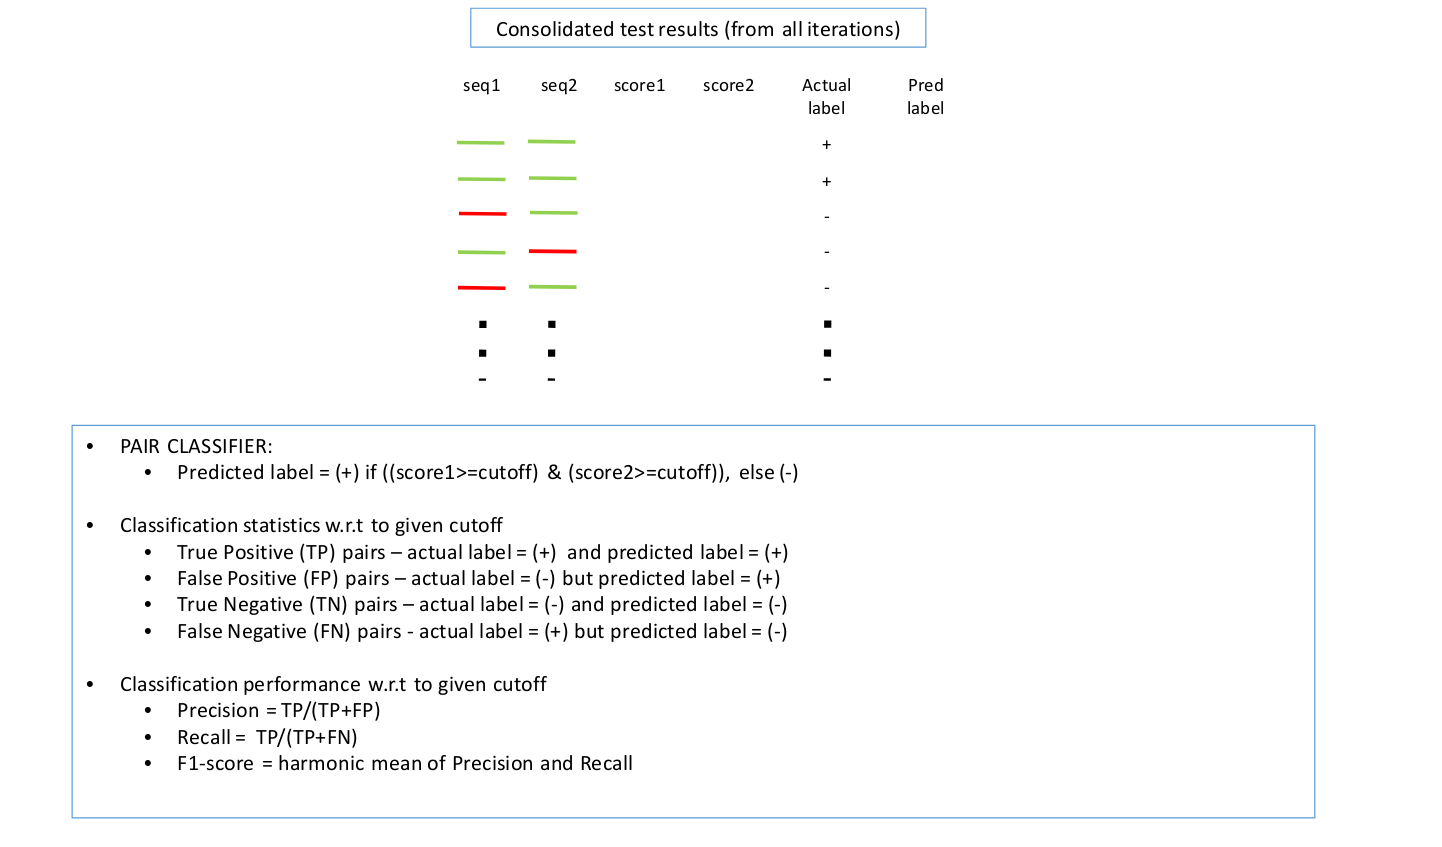
\includegraphics[width=\linewidth]{figures/train_classify2.png}}
				\caption{Evaluating pair classification model}
				\label{fig:train_classify2}
			\end{figure}
			
			\begin{figure}[h!]
				\fbox{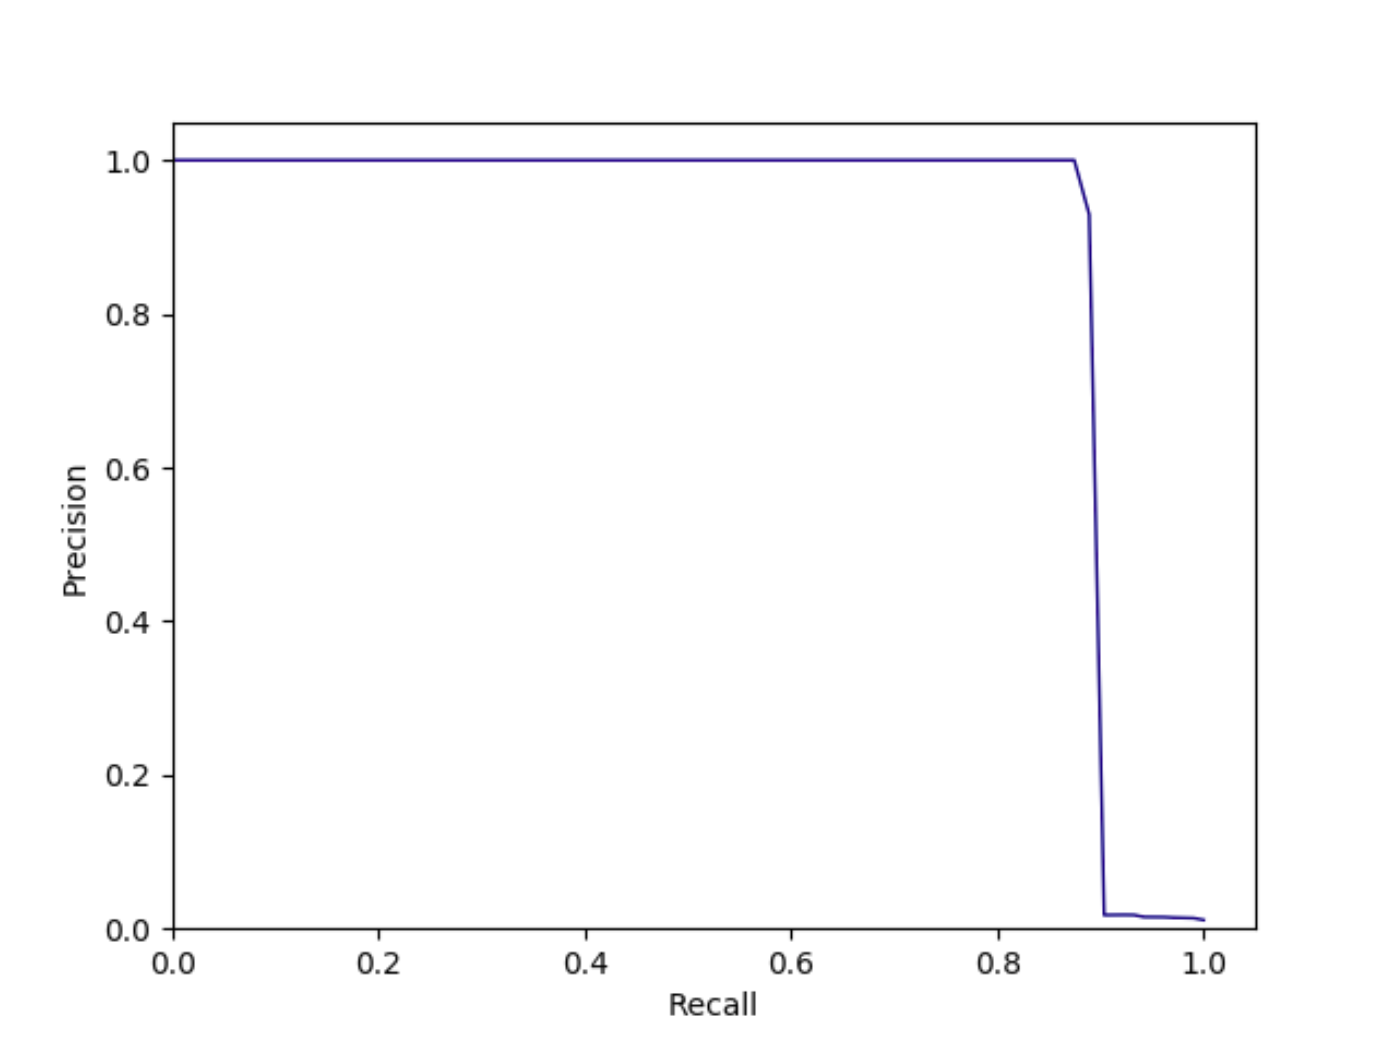
\includegraphics[width=\linewidth]{figures/test_PR-curve.png}}
				\caption{Example of PR-curve obtained during training}
				\label{fig:test_PR-curve}
			\end{figure}
		
			\subsubsection{Predicting missing sequences}
			Candidate missing sequences for every family are predicted using the non-family pairs. All the non-family pairs where the scores for both the sequences of a pair are greater than the best/lowest score cutoff are re-classified as positive pairs. Unique sequences within these reclassified positive pairs are predicted and reported as candidate missing sequences for the family.
			
		\subsection{Preliminary results}
		The pair classification based scoring was tested on 4796 yeast families from the Yeast Gene Order Browser (YGOB) database \citep{byrne2005yeast}. Since the YGOB families are built through manual curation using synteny based evidence, they were assumed to be "true". To check if the quality assessment workflow is assigning high quality scores to all the true families, the distribution of the PR-AUCs for all the 4796 yeast families was obtained (Figure ~\ref{fig:hist_pr-auc_true_ygob}). As expected the distribution of PR-AUCs is highly skewed towards PR-AUC value = 1.0 with 92\% of family classifiers having values $\geq$ 0.75. This shows that the method correctly recognizes good quality families and assigns high quality scores to them.
		
		\begin{figure}
			\fbox{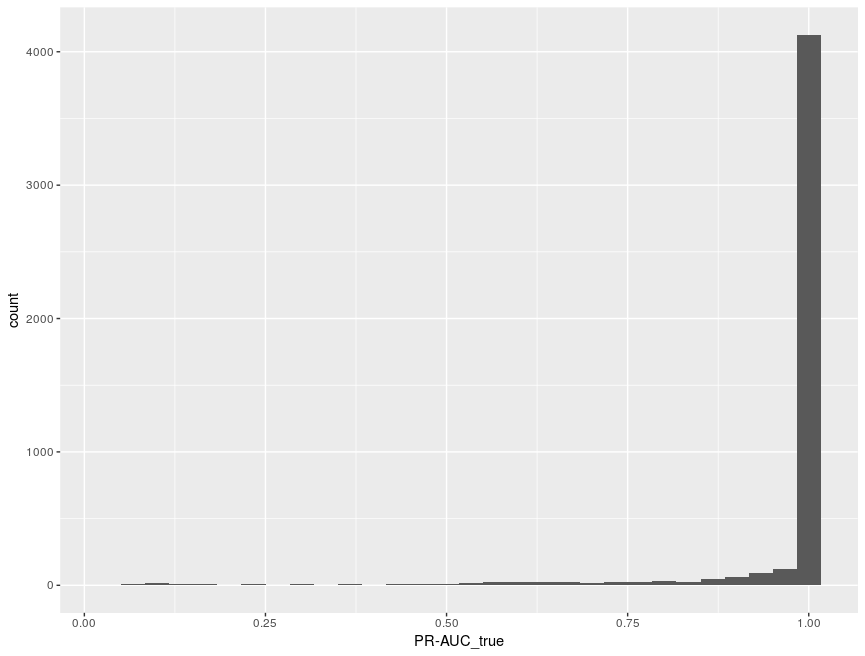
\includegraphics[width=\linewidth]{figures/hist_pr-auc_true_ygob.png}}
			\caption{Distribution of PR-AUC values for the true YGOB families}
			\label{fig:hist_pr-auc_true_ygob}
		\end{figure}
		
		\begin{figure}
			\fbox{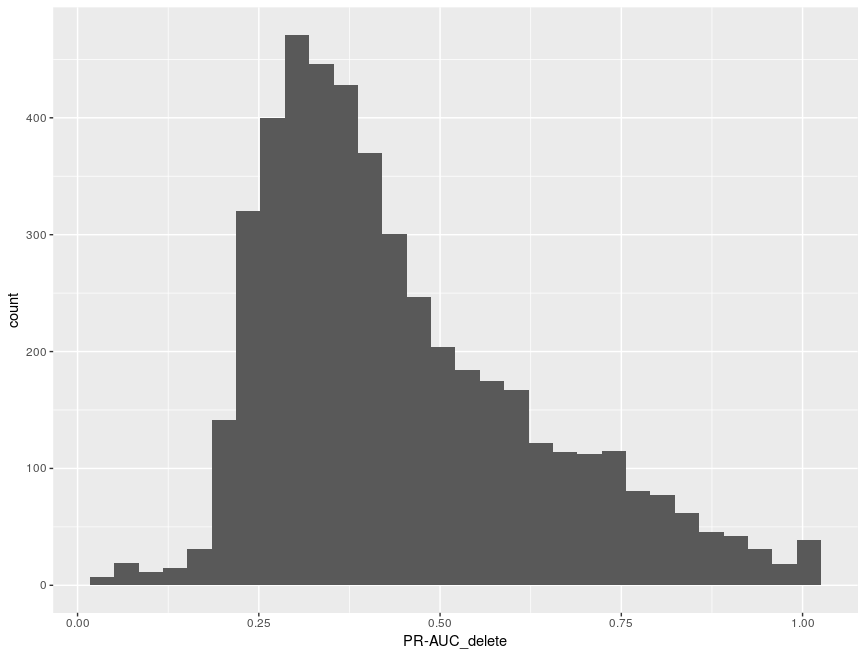
\includegraphics[width=\linewidth]{figures/hist_pr-auc_delete_ygob.png}}
			\caption{Distribution of PR-AUC values for the YGOB families with 20\% of sequences deleted}
			\label{fig:hist_pr-auc_delete_ygob}
		\end{figure}
		
		Even though the quality assessment method is proven to work on good/true families it is important to study the behaviour of the method on non-optimal families. To check the behaviour of the method on incomplete families, the true yeast families were artificially manipulated so that all the families are randomly missing 20\% of family sequences.
		
		The histogram in Figure ~\ref{fig:hist_pr-auc_delete_ygob} shows the distribution of PR-AUC values for 4796 artificially manipulated families where every family is missing 20\% of their sequences. A plot (Figure ~\ref{fig:scatter_pr-auc_true_vs_pr-auc_delete_ygob}) of true families PR-AUCs versus PR-AUCs after removing family sequences shows the drop in the PR-AUCs after removing family sequences from true families. The distribution indicates that the overall quality of the families drop significantly, which shows ability of method to detect incomplete families. Specifically, for 3971 out of 4796 families (83\%), the PR-AUC dropped significantly (PR-AUC$\geq$0.9 for true families and PR-AUC$<$0.75 after removing family sequences)
		
		\begin{figure}
			\fbox{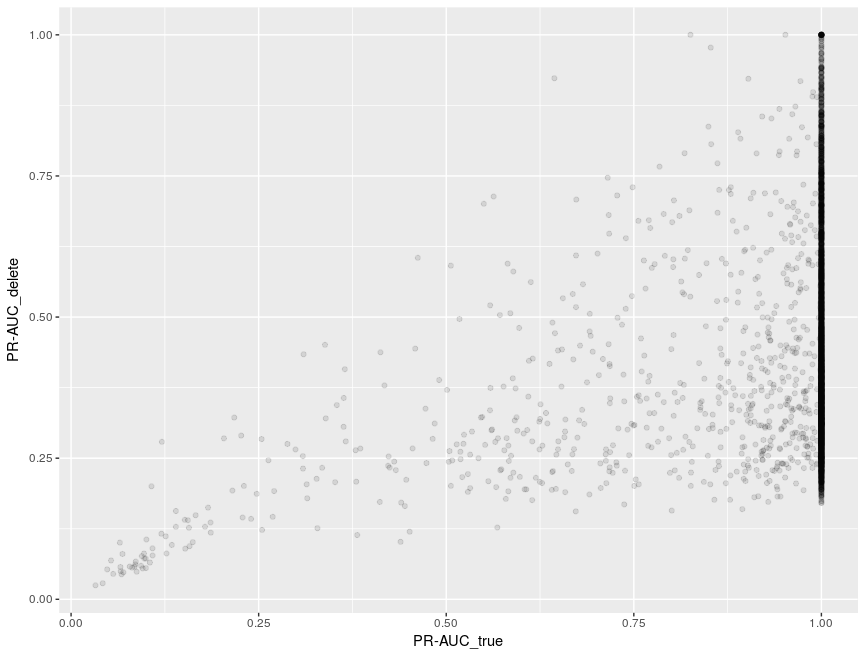
\includegraphics[width=\linewidth]{figures/scatter_pr-auc_true_vs_pr-auc_delete_ygob.png}}
			\caption{Plot of PR-AUCs obtained from true families versus PR-AUCs after deleting 20\% of sequences, for YGOB families}
			\label{fig:scatter_pr-auc_true_vs_pr-auc_delete_ygob}
		\end{figure}
	
		For each manipulated family, the missing sequences were predicted 
		back using lowest score cutoff obtained during training. The predicted missing sequences were compared to the true missing sequences and, precision and recall values were calculated to study the accuracy of predicted missing sequences. Precision was calculated as (TP/(TP+FP)) and recall was calculated as (TP/(TP+FN)) where True Positive (TP) are those predicted missing sequences that were truly missing from the family, False Positive (FP) are those that were predicted as missing but do not actually belong the family and False Negative (FN) are those that are truly missing but were not predicted as missing by the method. Out of 4796, the prediction performance for missing sequences was good (precision $\geq$ 0.75 and recall $\geq$ 0.75) for 3760 (78.4\%) families.
		
		\subsection{Signficance}
		This family scoring method assumes the given family to be under-clustered - the majority of sequences have diverged into the family - and attempts to build an HMM-based classifier that classifies pairs of sequences formed within the family from the pairs formed between family and the closest non-family sequences. The classification performance is mainly given by the PR-AUC value which shows how well the given family is separable from the closest families. This scoring method can be used in two ways; to characterize true families and to detect missing sequences for under-clustered families. For characterizing true families, the PR-curve and the PR-AUC can be used to see how well-behaved the family is in terms of its evolution. The best score cutoff obtained during training can be used to add sequences to the families from newly sequenced species. For under-clustered families, the PR-AUC is expected to be low as the precision value drops due to greater number of FP pairs (sequences trying to get in the family). The missing family sequences can be predicted using the best or the lowest score cutoffs depending upon preference of  high precision or high recall for prediction. If precision is preferred over recall then the best score cutoff can be used and if recall is preferred over precision then the lowest score cutoff can be used for predicting missing sequences.
		
		\subsection{Future work}
			\subsubsection{Merging small legume families}
			This scoring method will be used to inspect and merge small legume families into larger families. In the Ks-based legume families, there are approximately 2000 families that may be under-clustered ($\leq$10 family size). This will help in reducing the number of under-clustered families and generating a set of high-quality legume families.
			
			\subsubsection{Solving scalability issues}
			The pair classification based method is not fast enough to be efficiently applied on all legume the families. There are mainly two steps in the workflow that can be optimized to speed-up the method viz. the initial phmmer based database search and selecting the closest non-family sequences for forming negative pairs. Currently, every given family is searched against the entire set of all proteomes under study. The search space can be reduced by only searching within the neighborhood sequences/families.Tools like HHsearch \citep{soding2004protein} can be used to detect neighborhood families and limit the search space for every family. 
			
			Similarly, when selecting the closest non-family sequences, only those non-family sequences that are detected by more than one family sequences (or some proportion of family sequences) can be selected. Currently, a union of non-family sequences detected by every family sequence are selected for forming negative pairs.
			
			\pagebreak
	
	\section{Objective 2: Develop tree based and domain composition based methods for detecting over-clustered families}	
	\subsection{Tree based family scoring}
	Family trees are largely expected to follow the pattern of evolution from the species tree. This correspondence between gene trees and species trees has been used previously in multiple methods like TreeFam, LOFT, SYNERGY, ENSEMBLE 2007, PhIGs \citep{li2006treefam,van2007orthology,wapinski2007automatic,hubbard2006ensembl,dehal2006phylogenomic} for building gene families and detection of orthologs and paralogs from the family trees. Animal gene families in TreeFam are the group of genes evolved from a single gene in last common of all animals. Genes in one family are identified on the basis that they are phylogenetically separated by one or more genes from the outgroup species (S. cerevisiae, S pombe. or A. thaliana)
	
	Since gene families contain sequences that have diverged at or after the divergence of the earliest diverging species under study, genes within families have also diverged after the divergence of outgroup species. This evolutionary property of gene families can be used to score family trees by calculating the proportion of ingroup sequence pairs that appear to have diverged after the divergence of outgroup sequences in the corresponding phylogenetic trees of the families.
		\subsubsection{Methods}
		For a given rooted family tree, each pair of ingroup sequences, found within the tree, is labeled as True Positive (TP) or False Positive (FP) depending upon whether the pair appears to have diverged after or before the divergence of one or more outgroup sequences. A precision score for the family is calculated  as TP/(TP+FP) which gives the proportion of ingroup pairs diverging after the outgroup separation in the family tree.
		
		To check the divergence of any ingroup sequence pair in the tree, the Most Recent Common Ancestor (MRCA) of the pair is obtained. Then, all sequences corresponding to leaf nodes under this MRCA are collected. If this set of sequences contains one or more outgroup sequences, the corresponding ingroup pair is labelled as FP, else it is labeled as TP. The FP label for any ingroup pair indicates that there is atleast one outgroup sequence that has diverged after the divergence of the ingroup pair and the corresponding sequences of the pair have been wrongly clustered into one family. 
		
		\subsubsection{Preliminary results}
		This scoring method was applied on 18543 legume families. The Figure ~\ref{fig:hist_tree_precision_scores_lgf5} shows the distribution of scores across the legume families. Most of the families have higher precision scores ($\geq$0.75).
		
		To study the relationship between the tree based pair precision scores and family size, plot (Figure ~\ref{fig:scatter_tree_precision_vs_seqct_lgf5}) of precision scores versus number of ingroup sequences was obtained . As expected, most of families containing 15-45 ingroup sequences  have high precision scores. A considerable number of families, containing approximately 40 ingroup sequences, have tree precision scores around 0.5. These are the families where approximately half of ingroup pairs diverge after the divergence of one or more outgroup sequences. These families are prime candidates of over-clustered families. Also, large families with very low precision scores (majority of ingroup pairs have diverged before the outgroup divergence) may indicate problems with tree rooting.
		
		
		\begin{figure}[h!]
			\fbox{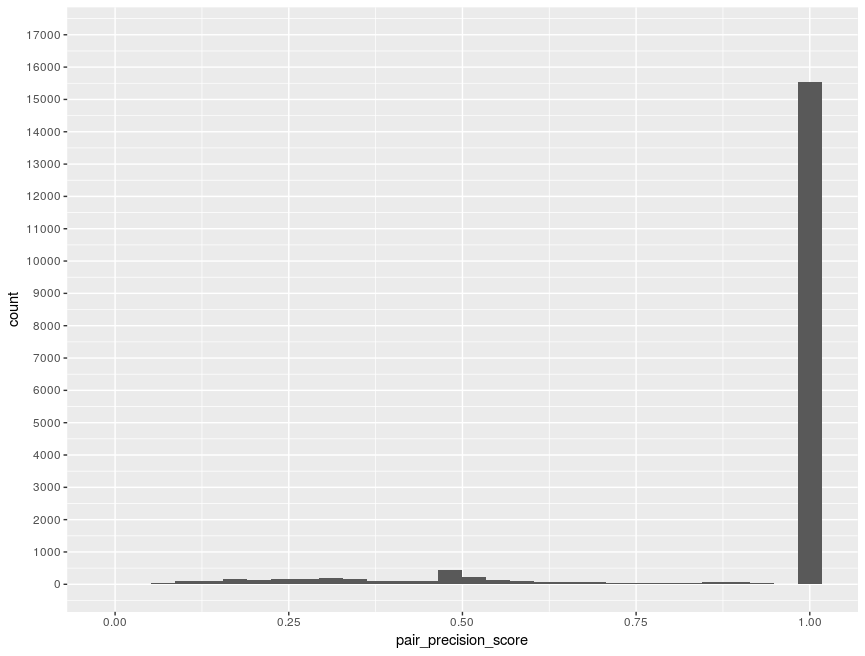
\includegraphics[width=\linewidth]{figures/hist_tree_precision_scores_lgf5.png}}
			\caption{Distribution of tree based pair precision scores for the Ks-based legume families}
			\label{fig:hist_tree_precision_scores_lgf5}
		\end{figure}
		
		\begin{figure}[h!]
			\fbox{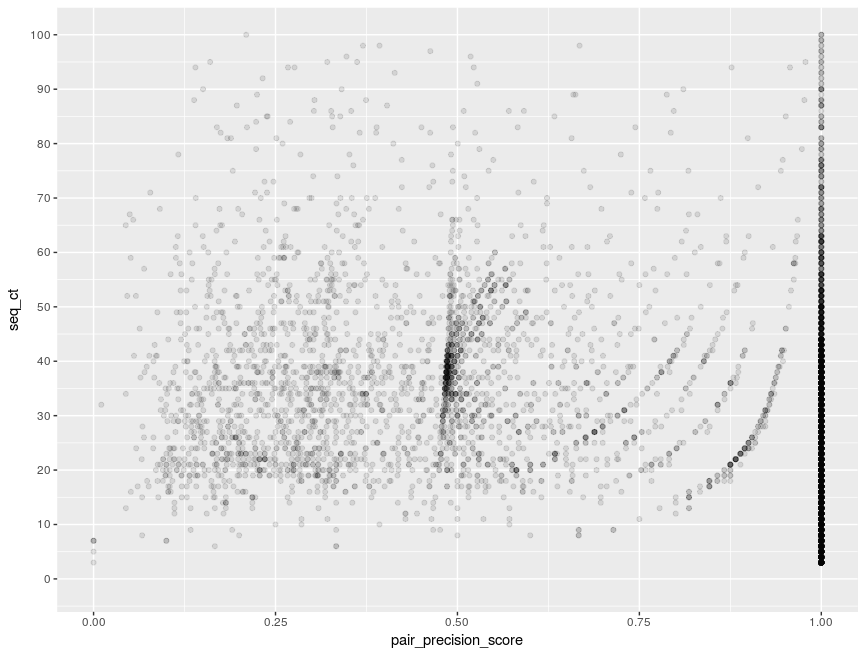
\includegraphics[width=\linewidth]{figures/scatter_tree_precision_vs_seqct_lgf5.png}}
			\caption{Plot of tree based pair precision scores versus ingroup sequence count for the Ks-based legume families}
			\label{fig:scatter_tree_precision_vs_seqct_lgf5}
		\end{figure}
		
		Examples of family trees with typical values of tree based pair precision scores are shown below. The outgroup sequences in the trees are shown in grey. Figure \ref{fig:tree_based_quality_type1_L_J5W12Z} shows family tree with low pair precision score (0.095). For this family, the majority of ingroup sequences do not form a monophyletic clade. Figure \ref{fig:tree_based_quality_type2_L_4L11VC} shows family tree with pair precision score = 0.507. This family has two monophyletic ingroup clades that could potentially be two ingroup families clustered together by the family building algorithm. This shows that the pair precision score can detect such over-clustered families. Finally, Figure  \ref{fig:tree_based_quality_type3_L_4VWLVV} shows a family with high pair precision score (0.876). Majority of ingroup  sequences form a monophyletic clade with two sequences diverging outside the family.
		
			
		\begin{figure}[h!]
			\fbox{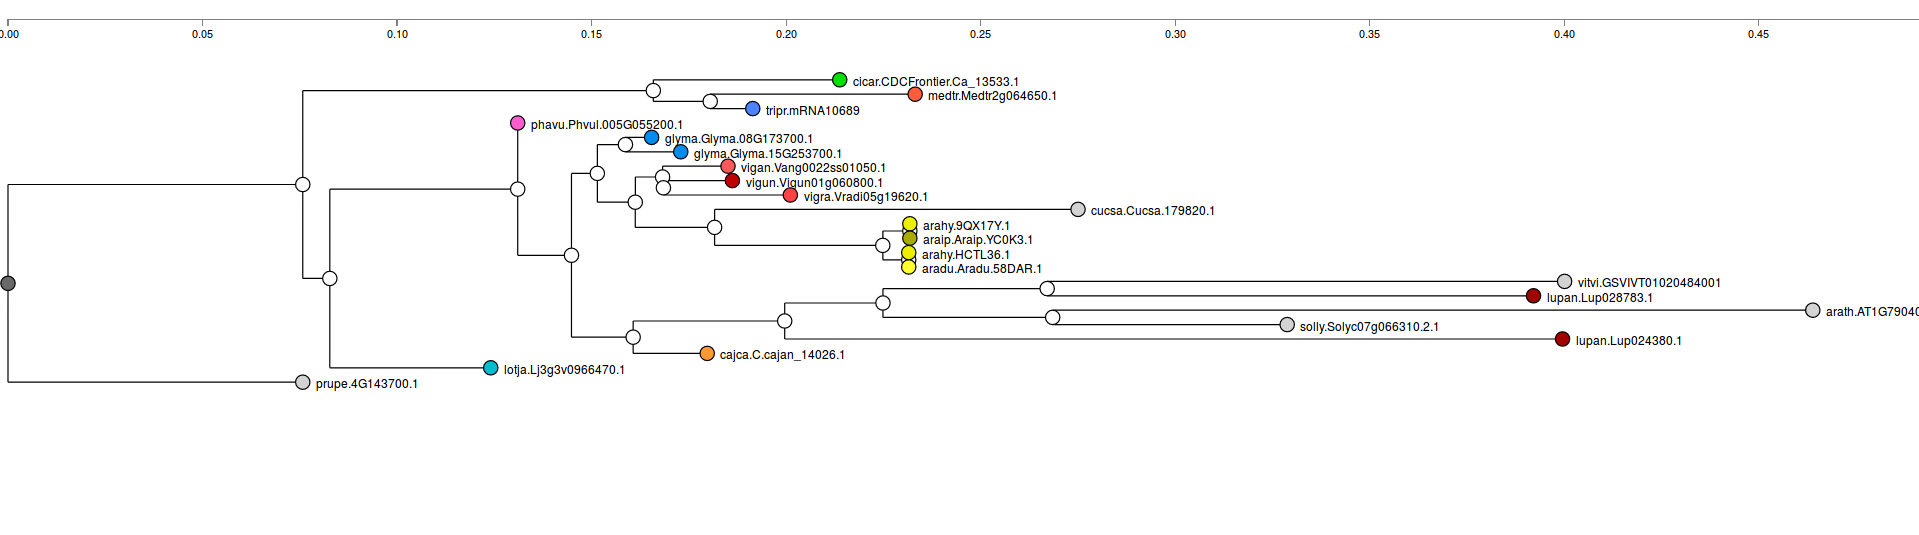
\includegraphics[width=\linewidth]{figures/tree_based_quality_type1_L_J5W12Z.png}}
			\caption{Example family tree with tree based pair precision score = 0.095}
			\label{fig:tree_based_quality_type1_L_J5W12Z}
		\end{figure}
		
		\begin{figure}[h!]
			\fbox{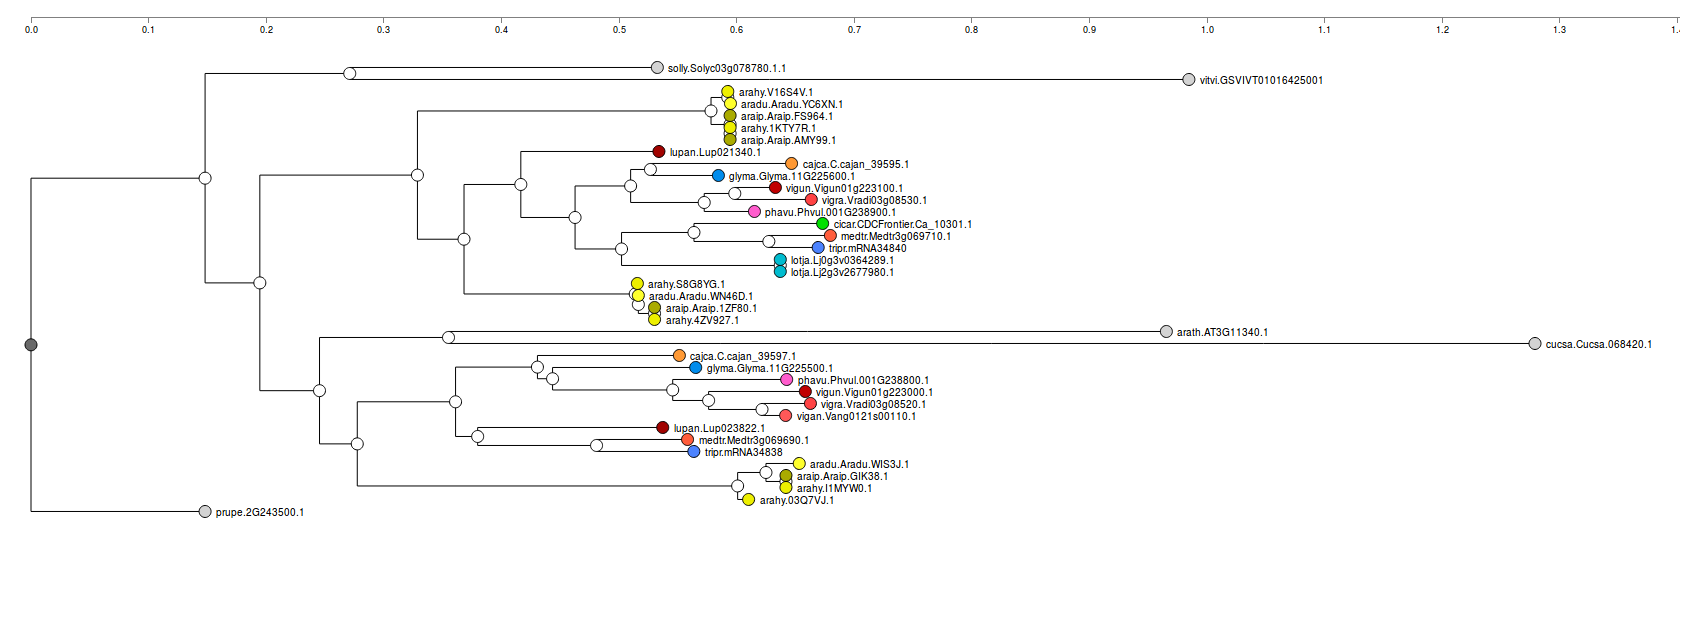
\includegraphics[width=\linewidth]{figures/tree_based_quality_type2_L_4L11VC.png}}
			\caption{Example family tree with tree based pair precision score = 0.507}
			\label{fig:tree_based_quality_type2_L_4L11VC}
		\end{figure}
		
		\begin{figure}[h!]
			\fbox{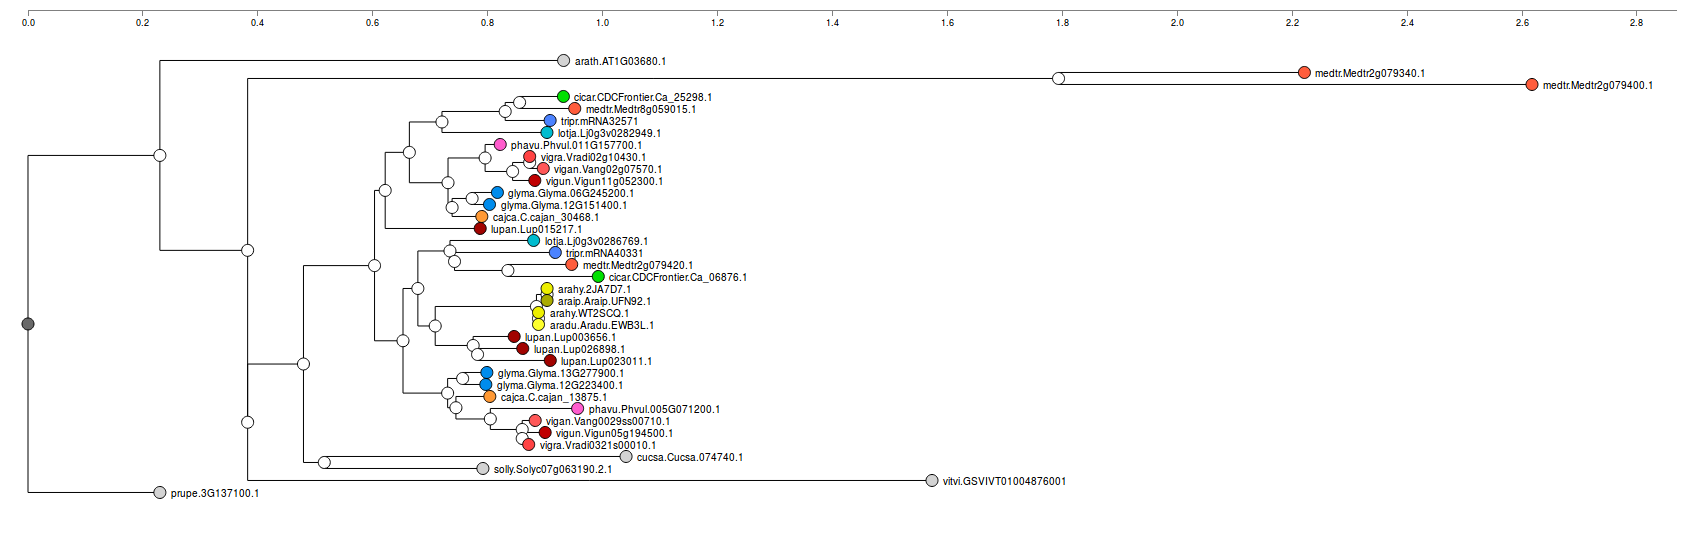
\includegraphics[width=\linewidth]{figures/tree_based_quality_type3_L_4VWLVV.png}}
			\caption{Example family tree with tree based pair precision score = 0.879}
			\label{fig:tree_based_quality_type3_L_4VWLVV}
		\end{figure}
		
		\subsubsection{Significance}
		This simple tree-based scoring method uses basic evolutionary properties of gene families to detect if all the sequences clustered in the family truly belong in the family, using the rooted evolutionary family tree. As seen from the preliminary results, this scoring method can be used to detect over-clustered families and family trees with rooting problems.
		
		
		\subsubsection{Future work}
		Over-clustered legume families detected using this method will be corrected to obtain a set of high-quality legume families. Also, large families with low precision scores will be re-rooted to maximize the precision scores.
		
		The merged families obtained using the pair classification based method will also be analyzed using the tree based scoring to resolve any over-clustered families produced due to merging.
		
		An R/Python tool can be developed where users can analyze and score family trees with respect to a given set of outgroups. The tool will also be able to directly extract ingroup clades from over-clustered families.
		\pagebreak
		
	\subsection{Domain composition based family scoring}
	Protein domains are sections of protein sequences that can fold and function independently. Consequently, multidomain proteins can evolve in a modular fashion through domain deletions/insertions/duplication in addition to sequence-based evolution. Databases like Pfam, PROSITE, SMART, CDD \citep{finn2007pfam,falquet2002prosite,letunic2011smart,marchler2010cdd} define and store domains detected in large number of protein sequences. Domain compositions/content have been previously used to detect sequence homology with high accuracies. \citep{song2007domain,bitard2015domain}. These were well separated gene families with distinctly different domain compositions (E.g. families separated at metazoan ancestor)
	
	Closely related sequences from the same family can be expected to have fairly similar domain types and domain content. Accordingly, this method assigns scores to given families based on number of domains shared between the sequences of the family. This scoring scheme will assign higher scores to family where most of the sequences have similar domain compositions. Good and well-conserved families are expected to have higher domain composition scores. Conversely, over-clustered families containing diverse sequences are expected to have lower scores due to less conservation of domain compositions across all the sequences.
	
	\subsubsection{Methods}
		\paragraph{Domain composition based jaccard score}
		For a given family, Pfam-A domains are assigned to all the sequences in the family using the pfamscan program \citep{mistry2007predicting}. The domains are assigned  to sequences in order of their start coordinates in the sequences. Then, for each pair of sequences in the family, A domain composition based Jaccard score is calculated using the function: $(n_1 \cup  n_2)/(n_1 \cap n_2)$, where $n_1$ and $n_2$ are the sets unique domains from sequence 1 and 2 of the pair, respectively. Jaccard score for the family is calculated as mean of all pairwise Jaccard scores from the family.
		
		\paragraph{Domain feature vector based cosine score}
		Here, the domain compositions of sequences within a given family are compared using their domain feature vectors. This is a new scoring method for comparing domain compositions of two sequences using their domain feature vectors. For example, consider two sequences X and Y from the same family having following domain order along the sequence, X: \{A,B,B,C\} and Y: \{A,A,B,D\}. The duplicate domains in both the sequences are assigned unique ids to distinguish them from each other, X: \{A, B, B-2, C\} and Y:\{A, A-2, B, D\}. The domain content universe for both the sequences is (A, A-2, B, B-2, C, D). Accordingly, the domain feature vector for both sequences is X: $(x_{1}, 0, x_{2}, x_{3}, x_{4}, 0)$ and Y: $(y_{1}, y_{2}, y_{3}, 0, 0, y_{4})$, where $x_{i}$ and $y_{i}$ are the alignment scores for the corresponding domain HMMs aligning against the sequences X and Y, respectively. Cosine similarities are calculated between all pairs of sequences using their domain feature vectors and the domain composition score for the family is calculated as the mean of all pairwise cosine scores.
		
		Pfam clusters closely related domains in Pfam-A into clans. For sequences within the same family, closely related domains could be  detected interchangeably, for same positions, in closely related family sequences. To avoid this, clan-ids of the domains are used instead of domain-ids for calculating the domain feature vector based cosine scores.
		
		\subsubsection{Preliminary results}
		The domain composition based Jaccard and cosine scoring were applied on the existing legume families to study the relationships between different scores and the ingroup sequence count. The score distributions for domain-based Jaccard scores can be seen from Figure ~\ref{fig:hist_domain_jaccard_scores_lgf5}.
		
		\begin{figure}
			\fbox{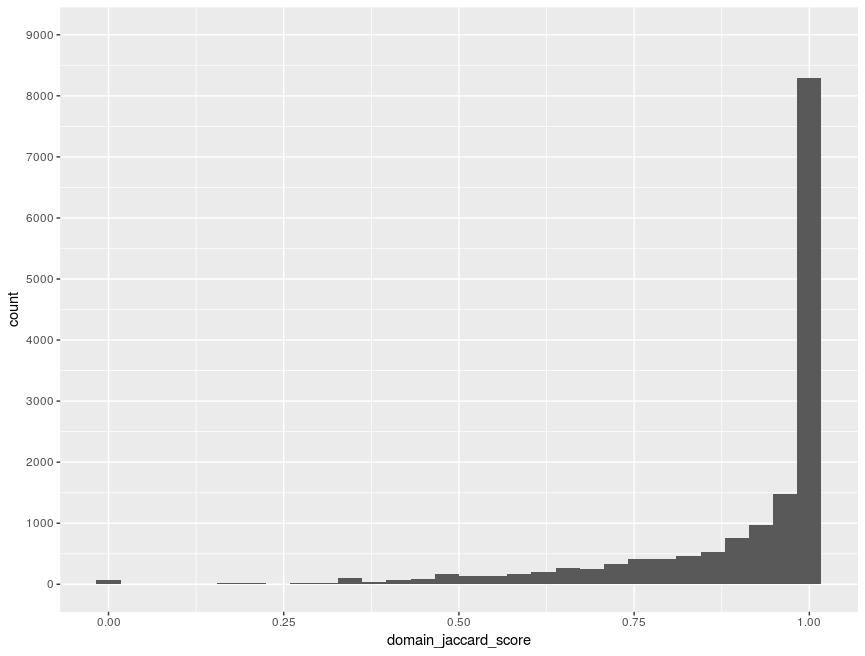
\includegraphics[width=\linewidth]{figures/hist_domain_jaccard_scores_lgf5.png}}
			\caption{Distribution of domain composition based Jaccard scores for the Ks-based legume families}
			\label{fig:hist_domain_jaccard_scores_lgf5}
		\end{figure}
		
		To study the relationship between the domain Jaccard score and family size, the plot of jaccard score versus number of ingroup sequences in the family was obtained (Figure ~\ref{fig:scatter_domain_jaccard_vs_seq_ct_lgf5}). The Jaccard scores are high for the majority of families in which the number of ingroup sequences is between 15-45.
		
		\begin{figure}
			\fbox{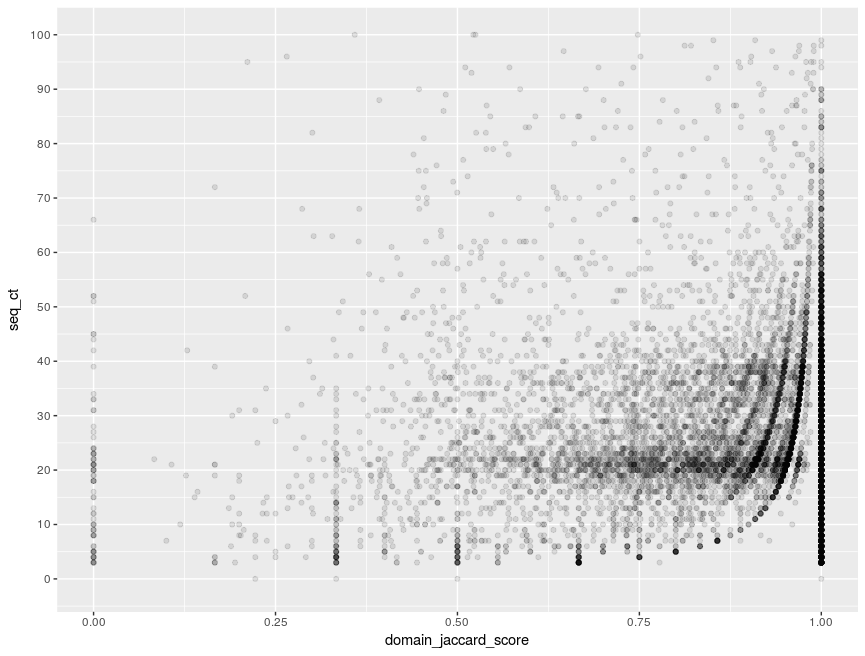
\includegraphics[width=\linewidth]{figures/scatter_domain_jaccard_vs_seq_ct_lgf5.png}}
			\caption{Plot of domain composition based Jaccard score versus ingroup sequence counts for the Ks-based legume families}
			\label{fig:scatter_domain_jaccard_vs_seq_ct_lgf5}
		\end{figure}
		
		The distribution of domain feature based cosine scores was also obtained (Figure ~\ref{fig:hist_domain_cosine_scores_lgf5}). Most of the families have high scores indicating that for a majority of the families, the domain compositions are fairly conserved. 
		
		\begin{figure}
			\fbox{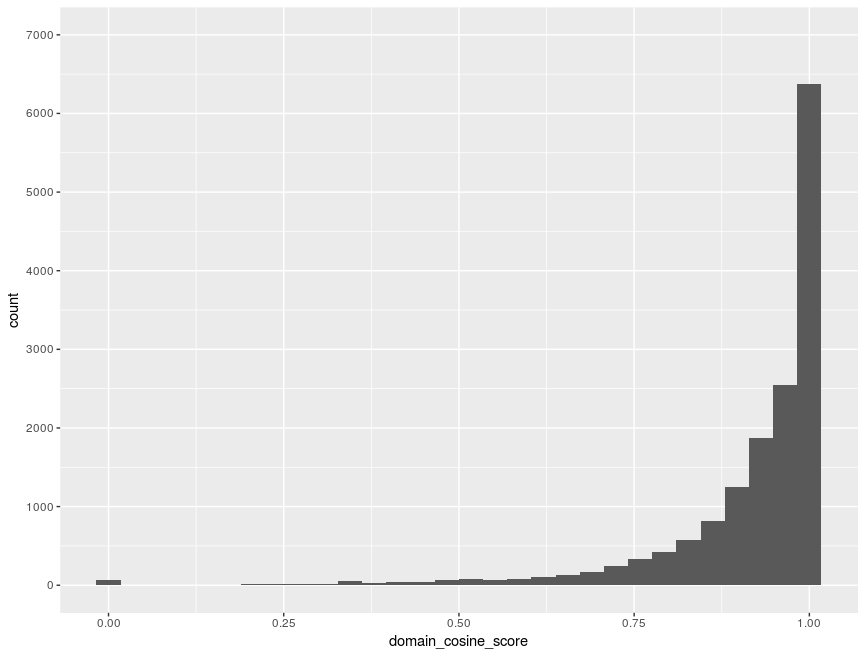
\includegraphics[width=\linewidth]{figures/hist_domain_cosine_scores_lgf5.png}}
			\caption{Distribution of domain composition based cosine scores for the Ks-based legume families}
			\label{fig:hist_domain_cosine_scores_lgf5}
		\end{figure}
		
		The plot (Figure ~\ref{fig:scatter_domain_cosine_vs_seq_ct_lgf5}) showing the relationship between the cosine score and family size was also obtained to study the relationship between cosine score and number of ingroup sequences in the family. Here, the scores correlate well (better than Jaccard scores) with family sizes, with higher scores for families with number of ingroup sequences between 15-45.
		
		\begin{figure}
			\fbox{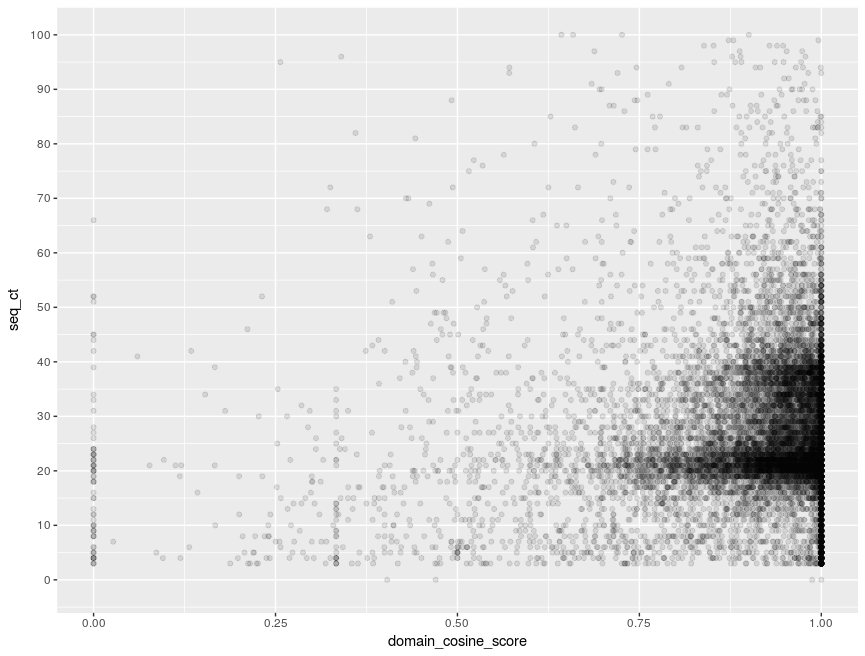
\includegraphics[width=\linewidth]{figures/scatter_domain_cosine_vs_seq_ct_lgf5.png}}
			\caption{Plot of domain composition based cosine scores versus ingroup sequence counts for the Ks-based legume families}
			\label{fig:scatter_domain_cosine_vs_seq_ct_lgf5}
		\end{figure}
		
		A plot (Figure ~\ref{fig:scatter_domain_cosine_vs_tree_precision_lgf5}) showing the relationship between the tree based pair precision scores and domain cosine scores was also obtained. The majority of families with high tree based precision scores also have high cosine scores. Specifically, for 11899 families, out of 15428 families, (77.1\%) both, the tree based pair precision scores and domain composition based cosine scores are $\geq$ 0.75.  In addition, two types of families can be seen from the plot; families with high tree based precision scores and lower domain scores and vice versa. The former are those that seem to evolve rapidly through domain insertion/deletion. The latter are those that seem to evolve slowly conserving domain compositions over longer evolutionary periods which could be the reason for the over-clustering.
		
		\begin{figure}
			\fbox{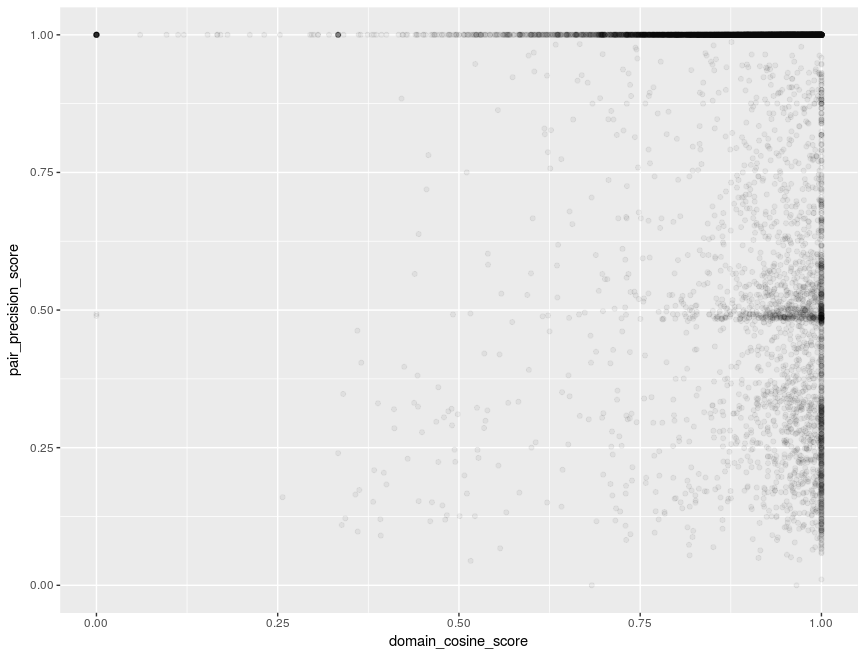
\includegraphics[width=\linewidth]{figures/scatter_domain_cosine_vs_tree_precision_lgf5.png}}
			\caption{Plot of domain composition based cosine score versus tree based precision scores for the Ks-based legume families}
			\label{fig:scatter_domain_cosine_vs_tree_precision_lgf5}
		\end{figure}
		
		Both the domain based family scoring methods have been developed into a Python tool that accepts the Pfam database and a directory containing family fasta files, and assigns domain composition scores to families.
	
	\subsubsection{Significance}
	Here we explore different domain based family scores mainly to detect over-clustering in families. Assuming that the species under study are closely related, the domain compositions for all the sequences in the family are expected to be largely conserved. The domain feature vector based cosine score seems to correlate better with family size and the tree based precision score as compared to the Jaccard score.
	
	The domain based scoring method can be used to detect candidate over-clustered families in conjunction with the tree based precision scores. This scoring method can also help in detecting rapidly evolving families.
	
	\subsubsection{Future work}
	Our scoring method will be used in the conjunction with the tree based precision score for detecting and improving  legume over-clustered families and for characterizing families. For example,  large families with low tree-based precision scores and low domain composition scores are prime candidates for over-clustered families. Also, large families with low tree-based precision scores and high domain composition scores are slowly evolving families that could be over-clustered due to their highly conserved domain architectures over longer evolutionary periods.
	
	It will also be interesting to study biological characteristics of families with high tree-based precision scores and low domain composition scores as these are the rapidly evolving families that have gained or lost protein domains within short evolutionary periods.
	
	
	\subsection{Species composition based family scoring}
	Species composition of a gene family can be defined as the number of sequences represented by per species in the family. Consistent/good families can be expected to have fairly even species compositions with most of the species represented in the family. Also, for well-behaved families the observed sequence counts, per species should be close to expected sequence counts per species. The expected sequence counts for each species per family is largely dependent on occurrences of large-scale duplications and deletions such as WGDs during species evolution.
		
		\subsubsection{Methods}
		For a given set of families, built from a specified set of species, a vector of expected species counts per family is obtained using expert opinion. This expected species count vector is compared to the observed species count vector from every family, using cosine similarity function (Equation ~\ref{cosine_sim_sp_comp}), to assign species composition based scores to corresponding family. Unusually small or large families with highly uneven species compositions are expected to have lower scores than families where most of the species are represented evenly.
		
		\begin{equation}
		cosine\_similarity(O,E) = \frac{O \cdot E}{\norm O \norm E}
		= \frac{\sum_{i=1}^{n} O_i E_i}{\sqrt{\sum_{i=1}^{n} O_i^2} \sqrt{\sum_{i=1}^{n} E_i^2}}
		\label{cosine_sim_sp_comp}
		\end{equation}
		
		\subsubsection{Preliminary results}
		The species composition based scoring  was applied to Ks-based legume families built from 14 ingroup legume species and 4 outgroup species. The expected count vector corresponding to the 14 legume species was inferred using the histories of the WGD detected in the evolution of the legume species. A WGD has occurred the common ancestor the legume species about 55 Mya (PGWD). Also, lineage specific  WGD and WGT have occurred in soybean and lupin, respectively. Moreover, the tetraploid peanut, \textit{Arachis hypogea} is an allopolyploid evolved for the two diploid Arachis species. Therefore, 4 soybean genes, 6 Lupin genes, 4 Arachis hypogea and 2 genes from rest of the 11 species can be expected to be present in families, assuming no gene loss during family evolution.
		
		The expected count vector was obtained as number of expected number of genes per species (Table  ~\ref{tab:exp_gene_count_table}). All the legume families were scored by comparing the expected counts vector to the observed species counts using cosine similarity function. The plot (Figure ~\ref{fig:scatter_famsize_vs_species_comp_cosine_score}) of species composition based family scores versus the ingroup sequence counts was obtained to study the relationship between family size that the scores. The plot shows that small families with highly uneven species composition have lower scores and the scores increase as the ingroup sequence count increases.
		
		\begin{table}[h!]
			\centering
			\begin{tabular}{|c |c |} 
				\hline
				Species ID & expected gene counts \\
				\hline\hline
				glyma & 4 \\ 
				\hline
				phavu & 2 \\
				\hline
				vigan & 2 \\
				\hline
				vigra & 2 \\
				\hline
				vigun & 2 \\ 
				\hline
				cajca & 2 \\
				\hline
				medtr & 2 \\
				\hline
				cicar & 2 \\
				\hline
				tripr & 2 \\
				\hline
				lotja & 2 \\
				\hline
				lupan & 6 \\
				\hline
				aradu & 2 \\
				\hline
				araip & 2 \\
				\hline
				arahy & 4 \\
				\hline
			\end{tabular}
			\caption{Expected gene counts per species per family, for legume families, assuming no gene loss following genome multiplications}
			\label{tab:exp_gene_count_table}
		\end{table}
		
		
		The legume families fall into at least 2 distinct size classes viz., families which seem to have lost the duplicate gene resulting from the Papilionoid WGD and those which seem to have retained the duplicate gene from the WGD. Families with ingroup sequence counts between 15-45 have highest composition scores with two distinct peaks between 15-30 and  30-45. These peaks correspond to the two types of legume families that have either lost or retained the PWGD duplicate.
		
		Minority of the largest families have high cosine scores.  These families have species counts that are far greater than expected, however, the composition is even across all the species. These families are likely result of gene-specific duplications that have occured in the common ancestor. This scoring method rightly assigns higher scores to these families.
		
		\begin{figure}[h!]
			\fbox{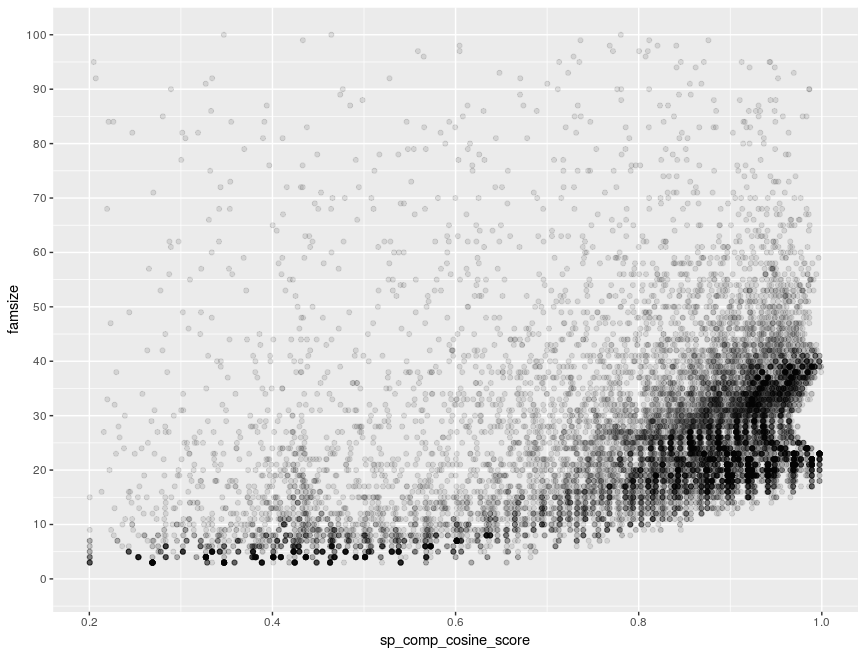
\includegraphics[width=\linewidth]{figures/scatter_famsize_vs_species_comp_cosine_score.png}}
			\caption{Plot of species composition based family scores versus the ingroup sequence counts of the Ks-based legume families}
			\label{fig:scatter_famsize_vs_species_comp_cosine_score}
		\end{figure}
		
		\subsubsection{Significance}
		The species composition based family scoring assumes that evolutionarily well-behaved families are expected to have sequence counts per species closer the expected sequence counts. The results on the legume families show that the scoring method assigns higher scores to legume families with sizes between 15-45 confirming the hypothesis that families between the range have even species compositions.
	
		\subsubsection{Future work}
		This scoring method can be used in conjunction with pair classification based, domain based and tree based scoring methods for correcting under-clustered and over-clustered legume families.Specifically, small/moderate families with low species composition score can be selected as under-clustered families for further processing through the pair classification approach.
		
		This scoring method can also be used for selecting legtimate ingroup clades while separating/cutting out family clades from over-clustered families detected using the tree based scoring method.
		
		
	\clearpage
	\section{Objective 3: Develop a workflow for building consensus families from multiple family sets}
	Family consistency can be assessed by comparing families generated by different family construction methods. This workflow involves comparing two sets of families, obtained from two different family building approaches, to establish family correspondences between the two sets - that is to determine which family from one set best corresponds to which family from the second set. Degrees of overlaps between corresponding families, between the two sets, can be used as measure of family consistency.
	
	The workflow is used to compare set of Ks-based legume families to a set of families obtained from OrthoFinder, to obtain a set of high-quality consensus families. OrthoFinder is one of the latest family building methods that is proven to beat popular family construction methods including OrthoMCL. The two sets are compared through their respective family HMM sets.
	
		\subsection{Methods}
			\subsubsection{Building HMM sets for families}
			Gene families are built from 11 legume proteomes with 2 outgroup proteomes, using the OrthoFinder algorithm. Similarly, legume families are also built using in-house Ks-based family building algorithm, from 14 legume proteomes with 4 outgroup proteomes. Two family HMM sets are obtained from both the sets of families using the hmmbuild program from the HMMER package.
			
			\subsubsection{Classifying common set of proteomes into families using HMM sets}
			A common set of 11 legumes proteomes with 2 outgroup proteomes are classified into both the family HMM sets using best matching family HMM strategy. Both HMM sets are searched against the common set of proteomes, using the hmmscan program from HMMER package. Each sequence is classified into any one family, from both the sets, for which the sequence aligns best (e-value $\leq$ 1e-5) with the corresponding family HMM.
			
			\subsubsection{Calculating family correspondence and family overlaps between the sets}
			For each family in both the sets, the largest overlapping family in the opposite set  is obtained. If, for example, $fam_1$ from $set_1$ is the largest overlapping family for $fam_2$ from $set_2$ and vice-versa, then $fam_1$ and $fam_2$ are considered corresponding families from both the sets. The two overlap scores, $fam_1-fam_2$ overlap and $fam_2-fam_1$ overlap are also calculated where $fam_1-fam_2$ overlap score is the proportion of sequences in $fam_1$ that overlap with $fam_2$ and, similarly, $fam_2-fam_1$ overlap score is the proportion of sequences in $fam_2$ that overlap with $fam_1$. If both the scores are 1.0 for a pair of families, then the two families match exactly from the two sets.
			
		\subsection{Preliminary results}
		The Ks-based and OrthoFinder legume family sets were compared using the family comparison workflow to explore the family correspondence between the two sets.
		
		There were 9160 families that were found to match exactly between both the sets (both overlap scores = 1.0). Eleven thousand five hundred fifty three families were found to match with more than 0.9 overlap score between both sets and 12934 families were found to match more that 0.8 overlap score.
		
		Both the overlap scores for each corresponding family pair from both the sets were plotted against each other (Figure ~\ref{fig:scatter_lgf5_vs_orthofinder_overlap_lgf5}). The families near the bottom right of the plot, on the y-axis, are those where the Ks-based family lies entirely within the corresponding orthofinder family. Similarly, the families near top left of the plot, on the x-axis,  are those families where the orthofinder family lies entirely within the corresponding Ks-based family.
		  
		\begin{figure}[h!]
			\fbox{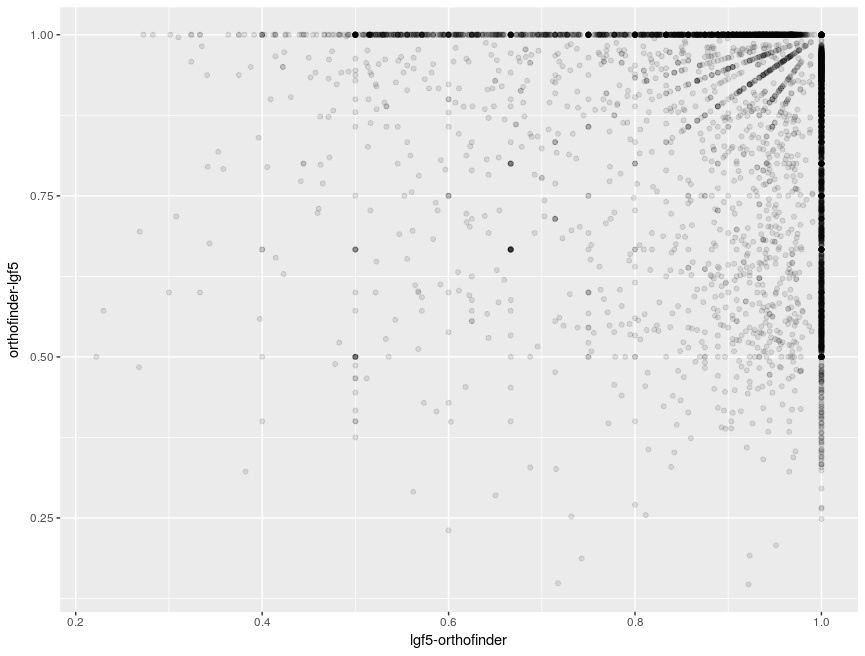
\includegraphics[width=\linewidth]{figures/scatter_lgf5_vs_orthofinder_overlap_lgf5.png}}
			\caption{Plot of the two way overlap scores obtained from comparison between the Ks-based and the OrthoFinder family sets}
			\label{fig:scatter_lgf5_vs_orthofinder_overlap_lgf5}
		\end{figure}
		
		\begin{figure}[h!]
			\fbox{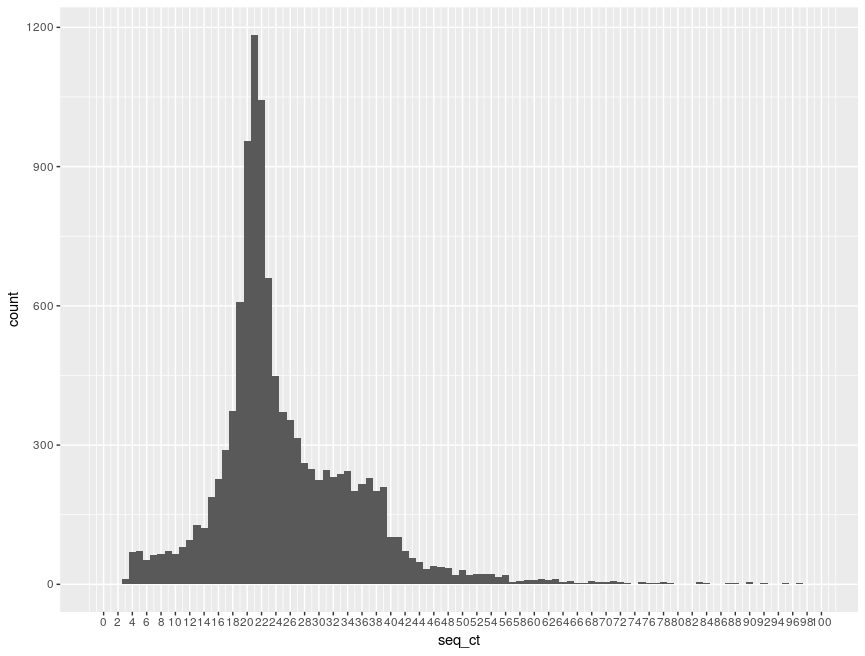
\includegraphics[width=\linewidth]{figures/hist_seq_ct_lgf5_vs_orthofinder_90percent_overlap.png}}
			\caption{Distribution of ingroup sequence counts for the Ks-based families with both overlaps scores $\geq$ 0.9 }
			\label{fig:hist_seq_ct_lgf5_vs_orthofinder_90percent_overlap}
		\end{figure}
		
		The distribution of ingroup sequence counts (Figure ~\ref{fig:hist_seq_ct_lgf5_vs_orthofinder_90percent_overlap}) was also obtained from the families where both the overlap scores were $\geq$ 0.9, to study the family size distribution of families that are consistently detected by both family building algorithms. The distribution shows that consist families are selected from all types of family sizes and not any particular family size.
				
		This workflow has been developed into a Python tool which accepts 2 sets of HMMs corresponding to the 2 family sets and a single set of sequences to be classified into the two family sets.
		
		\subsection{Future work}
		The legume families that are found to overlap between the two sets can be released as high-quality set of families. Different sets can be assigned different confidence levels according to the overlaps found between the two sets.
	
	\clearpage
	\section{Objective 4: Biological characterization of the legume families}
	This section involves exploring biological characteristics of different types of legume families. The legume ancestor is known to have undergone a WGD before divergence \citep{cannon2014multiple}.  However, some families seem to retain the duplicated gene and some families have lost the duplicate gene resulting from the WGD. As a result, legume families can be divided into distinct size classes - families with sizes between 10-30 and families between sizes 30-43. The former class of families are those that seem to have lost the duplicate gene and latter class have retained the duplicate gene. This work investigates if there is any biological basis to this phenomenon, using Gene Ontology (GO) enrichment analysis. 
	
		\subsection{Methods}
		Legume families are divided into 4 groups corresponding to the different size classes (marked by vertical lines in Figure ~\ref{fig:hist_lgf5_family_size_groups}) with group 1 containing families with sizes between 0-10, group 2 containing families with sizes between 10-30, group 3 containing families with sizes between 30-43 and group 4 containing families with sizes 43 and above. Due to exceptionally large number of families in group 2, a subset of families in group 2 is selected for further processing. The dashed lines show the subset of group 2 families.
		
		\begin{figure}[h!]
			\fbox{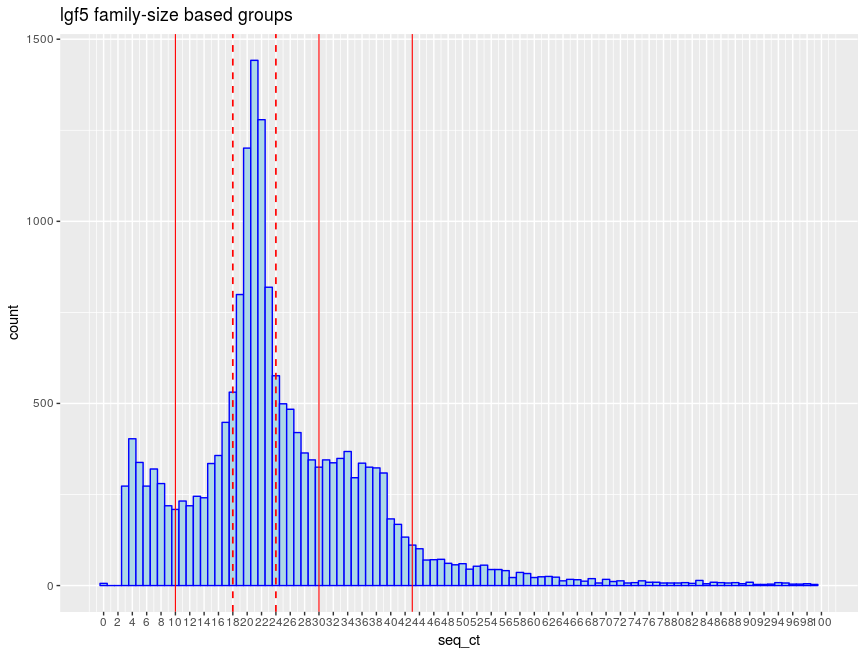
\includegraphics[width=\linewidth]{figures/hist_lgf5_family_size_groups.png}}
			\caption{Distribution of ingroup sequence counts for the Ks-based families}
			\label{fig:hist_lgf5_family_size_groups}
		\end{figure}
	
		Soybean (Glycine max) genes are extracted as representative genes from groups 1, 2-subset, 3 and 4, into separate lists. The gene lists are submitted for GO enrichment analysis on SoyBase \citep{grant2009soybase}. Enriched ontology terms are obtained for all 4 genes lists corresponding to the 4 family groups.
		
		\subsection{Preliminary results}
		Distinct GO terms were found to be significantly enriched for all 4 groups of families. The enrichment for group 1 was less significant. This may be because group 1 may contain fragmented under-clustered families that could be merged into families from other 3 groups. Tables ~\ref{tab:gotable_group1}, ~\ref{tab:gotable_group2_subset}, ~\ref{tab:gotable_group3}, ~\ref{tab:gotable_group4} show the top 5 enriched GO terms for each of the size groups.
		
		\begin{table}[h!]
			\centering
			\begin{tabular}{|c |c |c |} 
				\hline
				GO id & P-value & GO description \\
				\hline\hline
				GO:0009816 & $10^{-09}$ & defense response to bacterium, incompatible interaction \\ 
				\hline
				GO:0010026 & $10^{-05}$ & trichome differentiation \\
				\hline
				GO:0006355 & $10^{-04}$ & regulation of transcription, DNA-dependent \\
				\hline
				GO:0015690 & $10^{-03}$ & aluminum cation transport \\
				\hline
				GO:0009612 & $10^{-02}$ & response to mechanical stimulus \\ 
				\hline
			\end{tabular}
			\caption{GO enrichment for Group 1 soybean genes}
			\label{tab:gotable_group1}
		\end{table}
		
		\begin{table}[h!]
			\centering
			\begin{tabular}{|c |c |c |} 
				\hline
				GO id & P-value & GO description \\
				\hline\hline
				GO:0009658 & $10^{-45}$ & chloroplast organization \\ 
				\hline
				GO:0010027 & $10^{-45}$ & thylakoid membrane organization \\
				\hline
				GO:0019288 & $10^{-40}$ & isopentenyl diphosphate biosynthetic process \\
				\hline
				GO:0006364 & $10^{-37}$ & rRNA processing \\
				\hline
				GO:0019252 & $10^{-35}$ & starch biosynthetic process \\ 
				\hline
			\end{tabular}
			\caption{GO enrichment for Group 2 subset soybean genes}
			\label{tab:gotable_group2_subset}
		\end{table}
		
		\begin{table}[h!]
			\centering
			\begin{tabular}{|c |c |c |} 
				\hline
				GO id & P-value & GO description \\
				\hline\hline
				GO:0006355 & $10^{-92}$ & regulation of transcription, DNA-dependent \\ 
				\hline
				GO:0006468 & $10^{-25}$ & protein phosphorylation \\
				\hline
				GO:0010200 & $10^{-21}$ & response to chitin \\
				\hline
				GO:0010075 & $10^{-20}$ & regulation of meristem growth \\
				\hline
				GO:0009651 & $10^{-19}$ & response to salt stress \\ 
				\hline
			\end{tabular}
			\caption{GO enrichment for Group 3 soybean genes}
			\label{tab:gotable_group3}
		\end{table}
		
		\begin{table}[h!]
			\centering
			\begin{tabular}{|c |c |c |} 
				\hline
				GO id & P-value & GO description \\
				\hline\hline
				GO:0006952 & $10^{-191}$ & defense response \\ 
				\hline
				GO:0007165 & $10^{-66}$ & signal transduction \\
				\hline
				GO:0006412 & $10^{-54}$ & translation \\
				\hline
				GO:0055114 & $10^{-41}$ & oxidation-reduction process \\
				\hline
				GO:0006865 & $10^{-40}$ & amino acid transport \\ 
				\hline
			\end{tabular}
			\caption{GO enrichment for Group 4 soybean genes}
			\label{tab:gotable_group4}
		\end{table}
		
		
		
		\subsection{Future work}
		This analysis can be repeated on the high-confidence legume families obtained from the pair classification based family scoring workflow (merging under-clustered families), tree-based and domain-based scoring workflows (splitting over-clustered families) and the family sets comparison workflow (obtaining highly consistent families). 
		
		Applying domain based scoring on the high-confidence families can help in identifying slow-evolving/recent families (high Jaccard and cosine domain composition scores) and fast-evolving/ancient families (low Jaccard and cosine domain composition scores). GO enrichment analysis of these families can help in understanding the evolutionary pressures experienced by legume species during evolution.
		
		
	
	\bibliography{references/ref.bib}
	\bibliographystyle{apalike}
	
	
\end{document}